%%%%%%%%%%%%%%%%%%%%%%%%%%%%%%%%%%%%%%%%
\chapter{O Algoritmo \textit{PageRank}}%
%%%%%%%%%%%%%%%%%%%%%%%%%%%%%%%%%%%%%%%%

%Proposta do PageRank
O \textit{PageRank} é o principal algoritmo por trás das engrenagens de busca do \textit{Google}, criado em 1998 por Lawrence Page e Sergey Brin \ref{larry} para atribuir pesos a páginas da \textit{Web}. Ele tem como função atribuir um valor numérico para cada elemento em um conjunto de documentos, em que na \textit{Internet} tratariam-se de páginas \textit{Web}. Tendo como principal objetivo a identificação das páginas mais importantes aos usuários da rede, de forma a atribuir valores maiores as páginas mais importantes.

\
\begin{figure}[!htb]
	\centering
	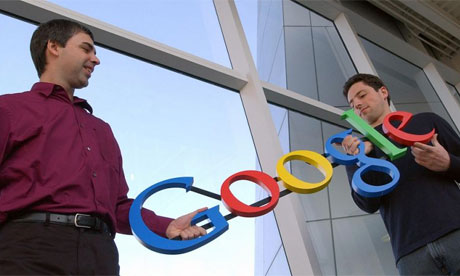
\includegraphics[scale=0.45]{imagens/larry}
	\caption{Lawrence Page e Sergey Brin criadores do \textit{PageRank} e fundadores do Google.}
	\label{larry}
\end{figure}

O \textit{Google} descreve o \textit{PageRank} da seguinte forma: \textit{"O \textit{PageRank} reflete nossa percepção de importância das páginas da \textit{Web} de forma a considerar mais de 500 milhões de variáveis e 2 bilhões de termos. Páginas que são consideradas importantes recebem um maior valor de PageRank, sendo assim, possuem maior possibilidade de aparecerem no topo de um resultado de busca."} 

%O grau de importância das páginas
A respeito da atribuição de importância às páginas, a página mais importante será a mais visitada e a página mais visitada será aquela que está associada a um maior número de \textit{links}. De forma mais precisa o número de visitas de uma página vai estar associado aos \textit{links} de saída que ela possui. Contudo, uma página também pode ser considerada importante por estar próxima a uma página de alto \textit{PageRank}. Algumas páginas famosas e seus \textit{PageRanks} são mostrados na tabela \ref{webrank}.


\vspace{0.3cm}

\
\begin{table}[!htb]
\centering
\begin{tabular}{lllll}
Nome da Página & PageRank\\
google.com & 10\\
ebay.com & 9\\
espn.com & 8\\
ge.com & 7\\
generalmills.com & 6\\
\end{tabular}
\caption{Valores atribuídos a algumas páginas da \textit{Web} pelo Google em 2007.}
\label{webrank}
\end{table}

%Google x PageRank
No trabalho em que foi proposto o \textit{PageRank} em 1998 \cite{brin2012reprint}, é resolvida a questão de como construir um sistema de larga escala para explorar informações adicionais da \textit{Web} de forma a lidar com coleções de páginas e \textit{links} não controlados, onde qualquer usuário da rede pode publicar ou retirar uma página a cada instante. 

Entretanto, o \textit{PageRank} é só uma pequena parte do sistema de buscas do Google. O sistema do buscador parte de uma \textit{query} que é feita na barra de pesquisa do Google \ref{google}, em seguida as palavras que estão contidas nesta \textit{query} são procuradas no conjunto de páginas indexadas pelo buscador. Por fim, o \textit{PageRank} faz o ranqueamento das páginas que possuem a palavra pesquisada.

\
\begin{figure}[!htb]
	\centering
	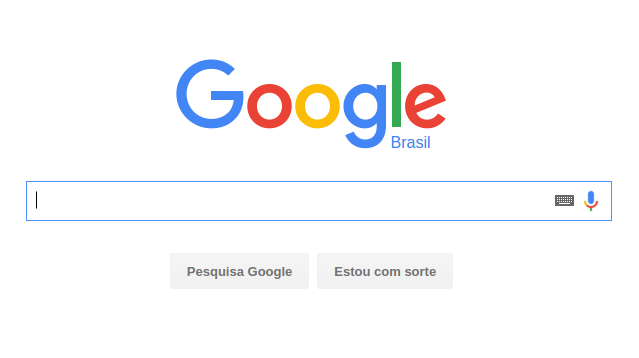
\includegraphics[scale=0.45]{imagens/google}
	\caption{Barra de pesquisa do Google.}
	\label{google}
\end{figure}

Contudo, apesar de toda a complexidade do sistema de busca, o maior problema por trás do buscador é fazer o ranqueamento desse número massivo de páginas. Não por acaso os fundadores escolheram o nome Google para representar a ferramenta de busca que haviam criado, uma vez que a palavra vem de googol, ou $10^{100}$, para representar a massividade da \textit{Web}. 


%%%%%%%%%%%%%%%%%%%%%%%%%%%%%%%%%%
\section{As Ferramentas de Busca}%
%%%%%%%%%%%%%%%%%%%%%%%%%%%%%%%%%%

O histórico de sucesso das ferramentas de busca está associado ao número de páginas indexadas pelos buscadores. Quanto mais páginas indexadas, melhores eram os resultados de busca pois estavam mais adequados ao que procurava o navegador. Desde 1994 tecnologias de busca têm tido que alcançar o crescimento da Web. Como pode-se constatar na tabela \ref{websize}, uma das primeiras ferramentas de busca, a \textit{World Wide Web Worm - WWWW} \cite{mcbryan1994genvl} possuia 110 mil páginas \textit{Web} indexadas. No entanto, em 1997 as melhores ferramentas de busca precisavam ter um índice com cerca de 100 milhões de páginas e em 1998 o Google surge com 518 milhões de páginas indexadas.

\vspace{0.3cm}

\
\begin{table}[!htb]
\centering
\begin{tabular}{lllll}
Ano & Buscador & Nº de Páginas Indexadas\\
1994 & WWWW & 110 mil\\
1997 & AltaVista & 100 milhões\\
1998 & Google & 518 milhões\\
2016 & Google & 4.8 bilhões
\end{tabular}
\caption{Número de páginas indexadas pelos buscadores.}
\label{websize}
\end{table}


%%%%%%%%%%%%%%%%%%%%%%%%%%%%%%%%%%%%%%%%%%
\section{O Problema do \textit{PageRank}}%
%%%%%%%%%%%%%%%%%%%%%%%%%%%%%%%%%%%%%%%%%%

O cálculo do \textit{PageRank} está sujeito a um grande problema, o custo computacional. Através dos dados apresentados na seção anterior, em função da grande dimensão da \textit{Web} pode-se constatar que esse cálculo não é nada trivial. Além do custo computacional, outros problemas surgem ao considerarmos os casos em que um navegador aleatório \cite{avrachenkov2007monte} não segue a estrutura de \textit{Hyperlink}. Assim, são três os principais problemas da simulação do cálculo do \textit{PageRank}: o problema dos \textit{Dark Holes} ou Buracos Negros, o problema da navegação descontínua por páginas não diretamente ligadas e o problema do cálculo do \textit{PageRank} de um conjunto massivo de documentos.

%Apresentação do modelo simples
O \textit{PageRank} pode ser pensado como um modelo que simula o comportamento de um usuário que age de forma aleatória. Considerar que existe um navegador que vai acessando páginas aleatoriamente, de forma a clicar somente em \textit{links} na página em que se encontra, consiste no modelo mais simples de cálculo do \textit{PageRank}. 

%Problema 1 - Buraco negro
Outra importante situação que precisa ser levada em consideração é a possibilidade de um usuário acessar uma página sem links de saída, como por exemplo, um link que o direcione para um documento PDF, como ilustrado na figura \ref{blackhole}. Neste caso o usuário poderia usar o botão de voltar do \textit{Browser} para sair deste tipo de buraco negro na rede, o que simplifica possíveis problemas no cálculo do \textit{PageRank}.  

\
\begin{figure}[!htb]
	\centering
	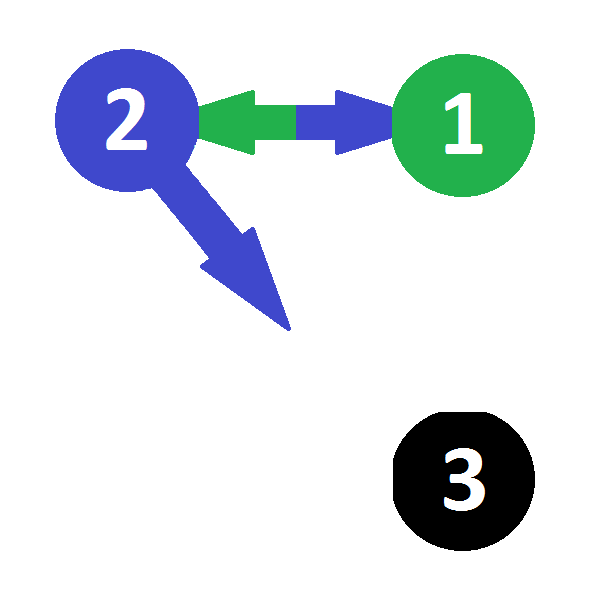
\includegraphics[scale=0.35]{imagens/blackhole1}
	\hspace{0.1cm}
	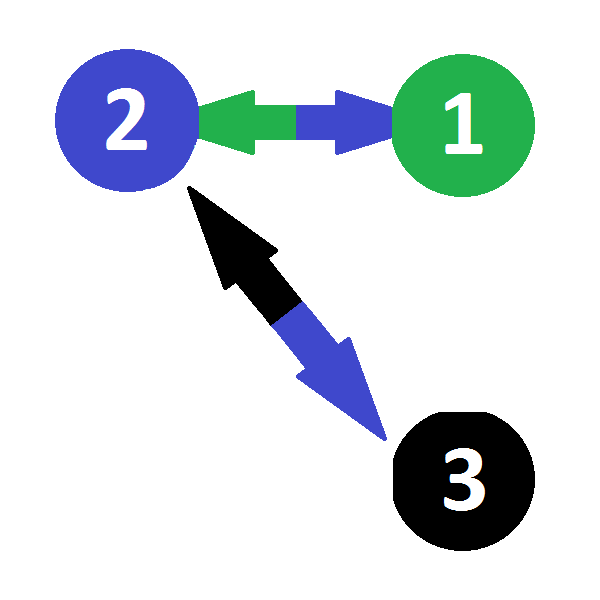
\includegraphics[scale=0.35]{imagens/blackhole2}
	\caption{O buraco negro da \textit{Web}.}
	\label{blackhole}
\end{figure}

%Problema 2 - Teleportation Model
Um outro problema surge ao considerar-se que o usuário pode saltar de uma página para outra sem seguir a estrutura de \textit{links}, por ficar entediado, ou por um outro motivo qualquer. Um exemplo de como isso poderia ocorrer, é o caso do usuário estar na página do Laboratório Nacional de Computação Científica - LNCC e seguindo a estrutura de \textit{Hyperlink}, clicar em um \textit{link} que o leve à página do governo federal. No entanto, o usuário de repente altera o \textit{Uniform Resource Locator - URL} e vai para um \textit{site} de notícias que não está diretamente ligado aos outros dois \textit{sites}. Este exemplo é ilustrado na figura \ref{tele}.

\
\begin{figure}[!htb]
	\centering
	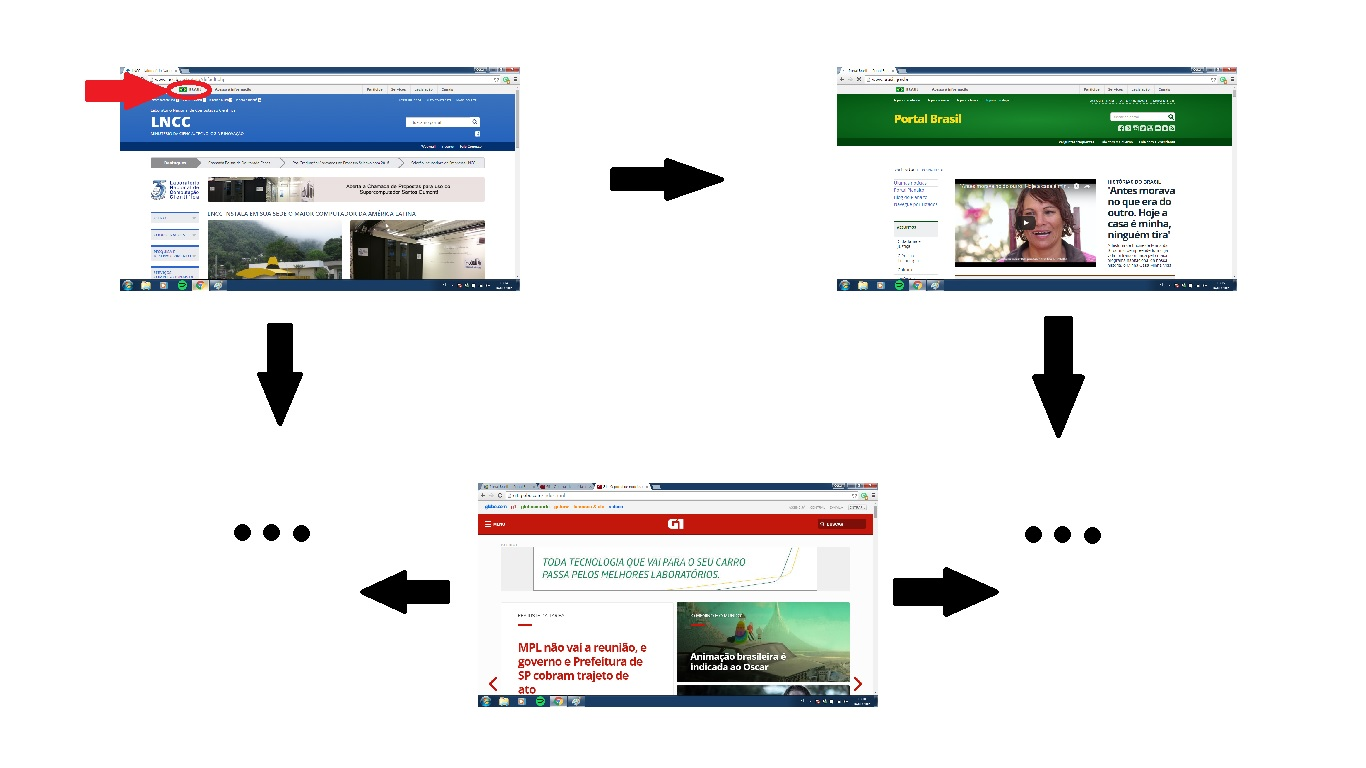
\includegraphics[scale=0.3]{imagens/tele}
	\caption{Navegação entre páginas indiretamente conectadas.}
	\label{tele}
\end{figure}

\noindent Este problema foi apontado pela primeira vez no artigo que deu origem ao Google em 1998 \cite{brin2012reprint}, e foi recentemente apelidado em \cite{ishii2014pagerank} de \textit{Teleportation Model}.

%Problema 3 - A massividade da Web
A massividade da \textit{Web} é uma das principais questões por trás do cálculo do \textit{PageRank}, considerando que a dimensão da \textit{Web} pode tornar o ranqueamento de páginas impossível. No entanto, a solução para este problema é o uso de algoritmos distribuídos, sobre os quais a cada ano novas publicações são feitas \cite{lei2015distributed}. Neste contexto, a fim de melhorar a performance do processamento, o cálculo a partir do modelo distribuído é realizado com a ajuda de vários conputadores num \textit{cluster}, como o da figura \ref{cluster}. Sendo assim, os recursos computacionais já necessários para abrigar a \textit{Web} também seriam usados para o cálculo de \textit{PageRank}.    

\
\begin{figure}[!htb]
	\centering
	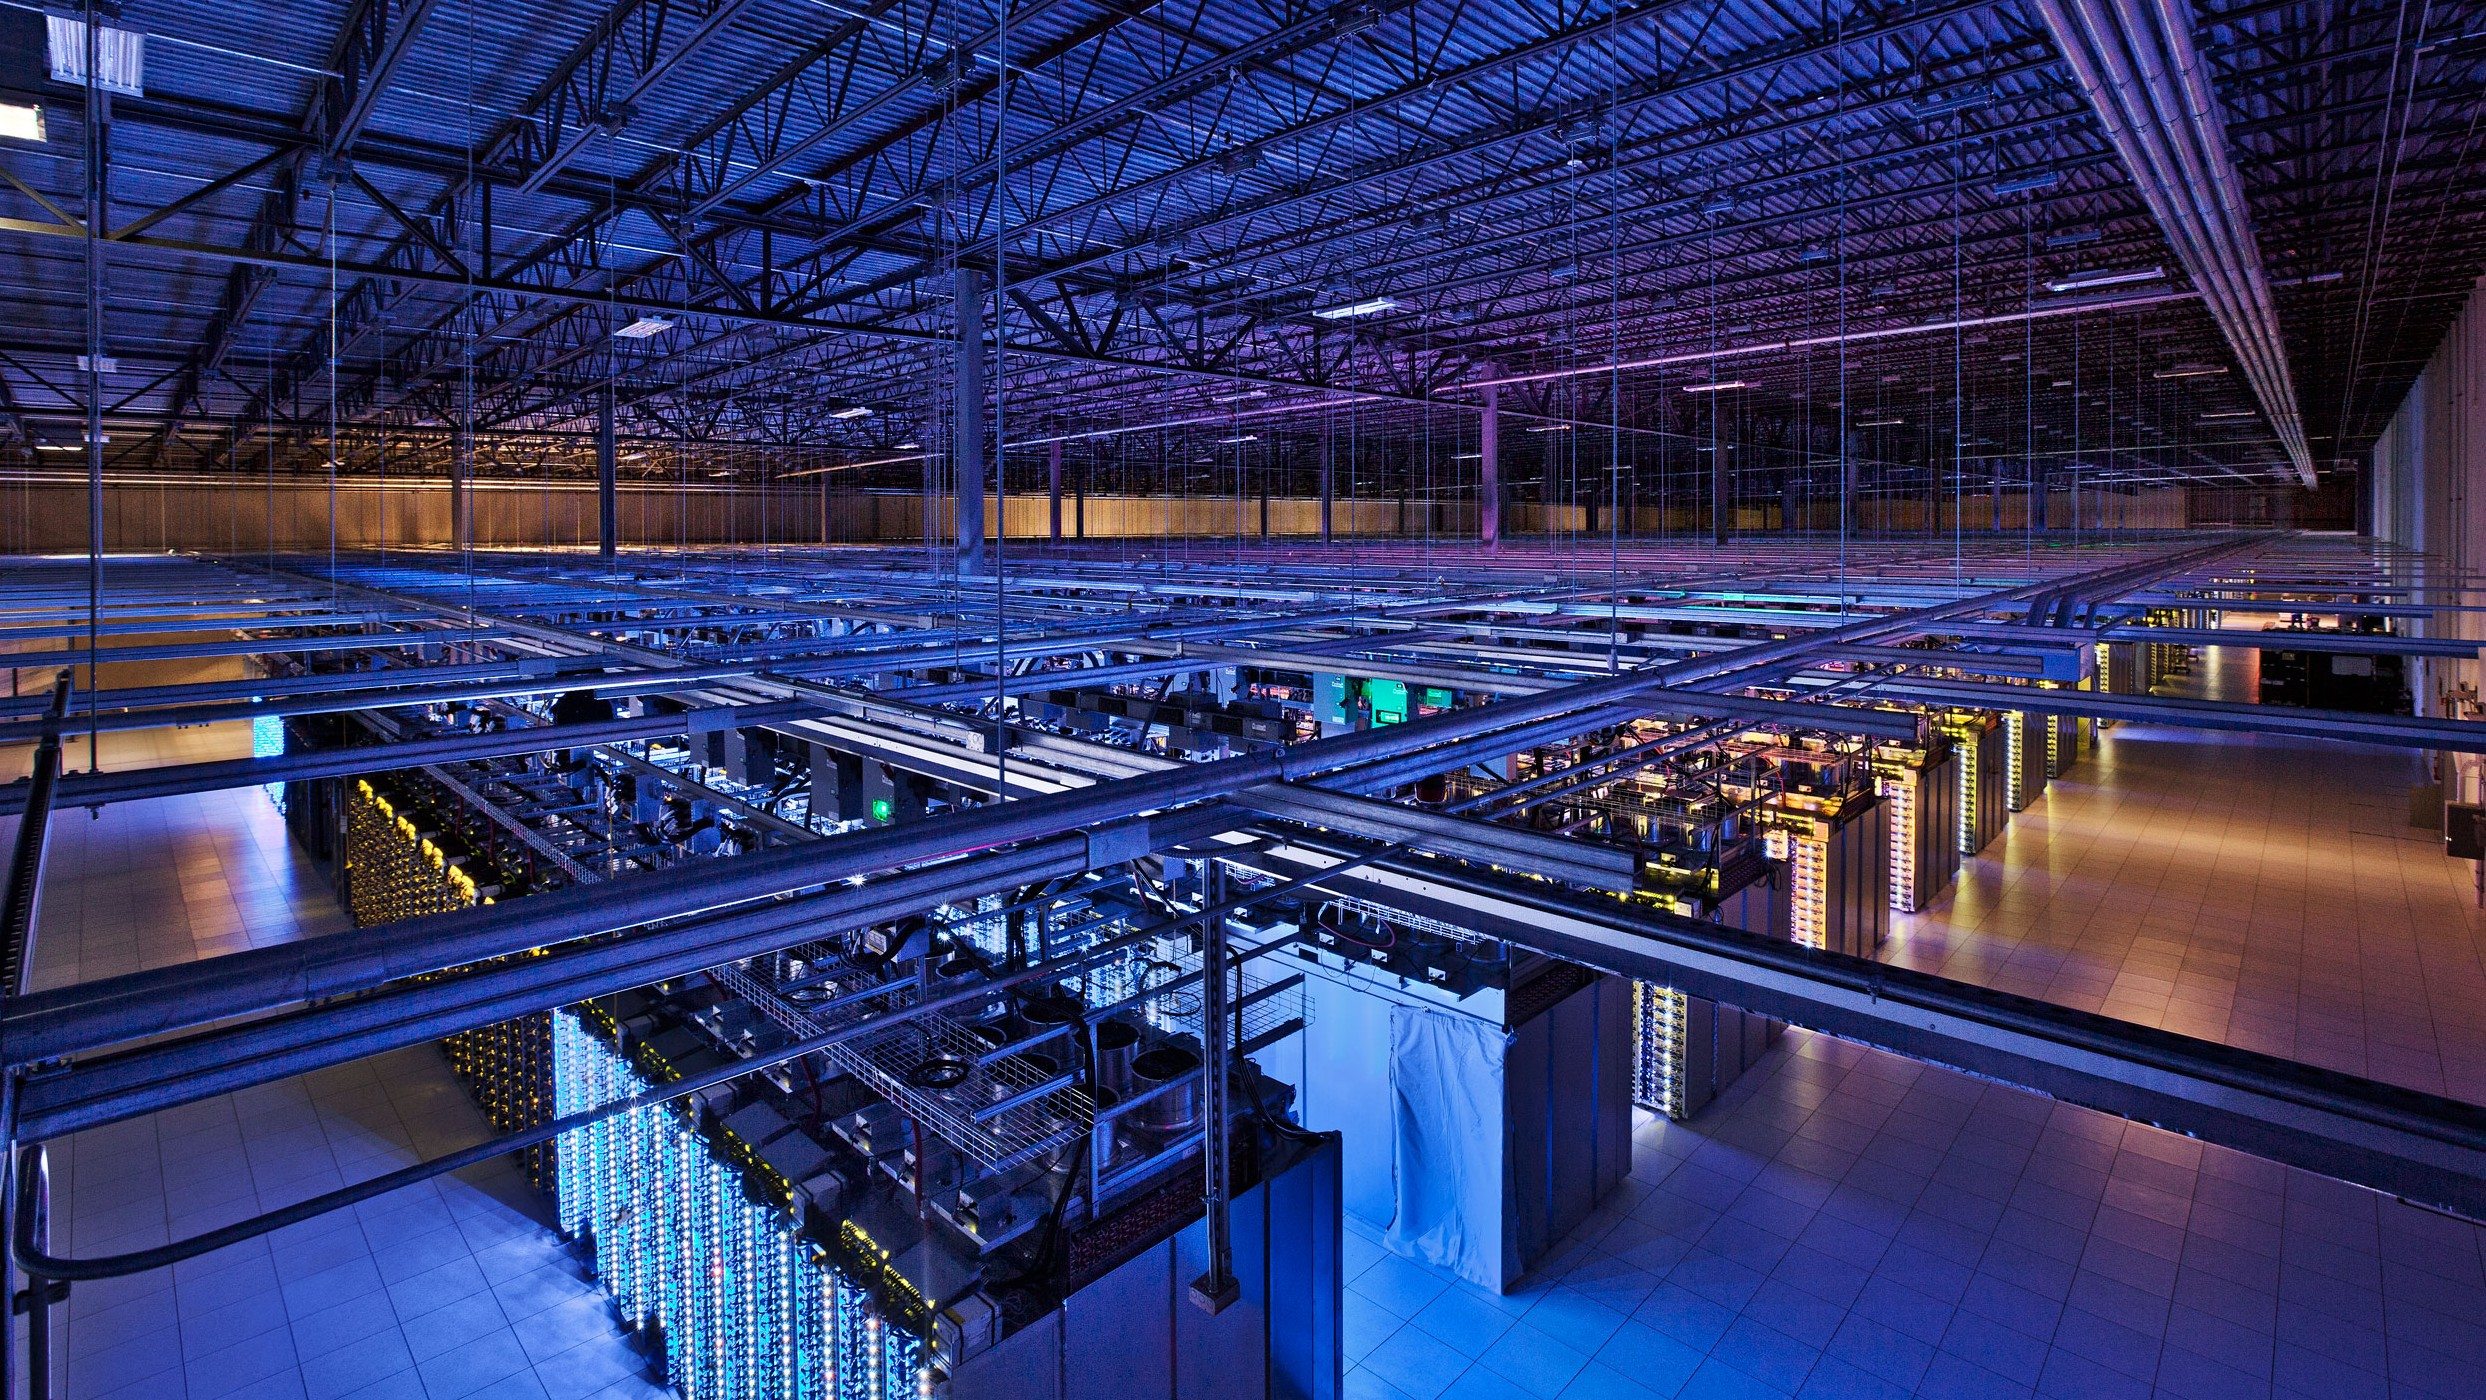
\includegraphics[scale=0.1]{imagens/cluster}
	\caption{Cluster do Google.}
	\label{cluster}
\end{figure}